\section{Benchmarks}
\label{sec:benchmarks}

\subsection{Overview}
\label{sec:bench_overview}

\macaron{} is evaluated on three groups of benchmarks, each with a different evidentiary role. The internal Personal Intelligence benchmarks (\chatbench{} and \livingbench{}) measure fit to the conversational and stateful-agent behaviors targeted by the L0 and L1 specialists. \uifora{}-Bench holds the \uifora{} runtime, case set, viewports, judge, and scoring policy fixed across models, and evaluates their ability to generate clear, accurate, interactive interfaces in that shared environment. \venti{} is evaluated with L3 as part of its released model system, while the runtime itself is common evaluation infrastructure. The general-capability suite samples tasks that test transfer to agent and coding settings. Where matched base-model measurements are available, they provide a regression check, but the suite as a whole is not a formal non-regression guarantee.

The Personal Intelligence benchmarks share a design problem that sets them apart from standard correctness benchmarks. Quality judgments for personalized experience depend on the joint context of user identity, interaction scenario, and relationship stage. The same model behavior may warrant different optimal judgments under different conditioned contexts, making context-free objective correctness difficult to define~\citep{manheim2018,stanfordreglab2025}.

This property gives rise to two interrelated evaluation challenges. First, experience quality within a conversation is dispersed across conversational nuances, and the same behavior may carry different implications for different users and scenarios. Fixed rubrics alone can under-specify these conditional judgments~\citep{thoppilan2022,bowman2021,zheng2023,mehri2020,dubois2024}. Second, personal-assistant behavior unfolds as requirements, world state, and available information change. The model must integrate partial information, revise plans, and operate within the user's limited patience. These dynamics are difficult to capture with static or single-turn evaluations~\citep{raji2021,kiela2021,lin2024,xie2024}.

We operationalize these challenges through experience--model co-design. Real interactions and product failure analyses supply candidate behaviors; the benchmark formalizes them into executable evaluation logic; and evaluation artifacts can in turn supply candidates for later training. \macaron{} implements this path from interaction evidence to evaluation logic and training-sample generation. This coupling is useful for product iteration, but it also makes the internal benchmarks less independent of the training process than a frozen external test set.

\chatbench{} (Section~\ref{sec:chatbench}) turns context-dependent experience-quality judgment into reproducible conditioned evaluation, making subjective conversational quality amenable to structured assessment. \livingbench{} (Section~\ref{sec:livingbench}) brings dynamically unfolding multi-turn behavior into controlled simulation under realistic noise, so that dynamic capabilities such as state maintenance and replanning can be observed and scored.

\paragraph{Scope and comparison protocol.}
The three internal evaluations are curated suites comprising 46 \chatbench{} cases, 40 \livingbench{} scenarios, and 161 \uifora{}-Bench cases (Appendix~\ref{app:eval_protocols}). Within each benchmark, every unstarred model is evaluated on the same case set with the same benchmark-specific simulator or harness, judge stack, sampling policy, and aggregation rule, and this common per-benchmark protocol grounds direct comparison within each row. \chatbench{} and \livingbench{} share source domains and failure taxonomies with the RSI loop, so they characterize performance on the targeted Personal Intelligence distribution, while the external benchmark suite provides complementary coverage. All three use LLM-mediated judgment for at least part of the score, with versioned deterministic aggregation and retained run artifacts where applicable.


\subsection{Personal Intelligence Benchmarks}
\label{sec:pi_benchmarks}

\chatbench{} and \livingbench{} are the two Personal Intelligence benchmarks. Both exercise interaction trajectories rather than isolated answers, targeting conversational behavior and stateful-agent behavior respectively. The broader suite in Section~\ref{sec:general_bench} provides a complementary transfer check under the protocol defined for each benchmark.

\subsection{\chatbench}
\label{sec:chatbench}

\chatbench{} evaluates the quality of collaborative experience in single conversations through context-conditioned judgment. Because this quality varies with user identity and conversation scenario, the benchmark fixes a common set of axioms and scenario types while allowing the judge to instantiate case-specific criteria from the supplied persona and context. The resulting score remains an LLM-mediated judgment rather than an objective correctness measure.

\subsubsection{Judgment Criteria}
\label{sec:chatbench_axioms}

Static rubrics can miss context that changes how a behavior should be interpreted. \chatbench{} therefore adopts a dynamic constitutional structure, fixing six axioms across the benchmark while the judge derives case-specific criteria from the user persona and scenario. Table~\ref{tab:axioms} lists the fixed axioms.

\begin{table}[ht]
\centering
\caption{Six constitutional axioms for dynamic quality derivation.}
\label{tab:axioms}
\begin{tabularx}{\textwidth}{@{}L{0.20\textwidth}Y@{}}
\toprule
\textbf{Axiom} & \textbf{Definition} \\
\midrule
Felt Understanding & The user senses that their intent, state, and unspoken needs are grasped \\
Honest Counsel & The model holds its own position rather than bending to please \\
Authentic Voice & Expression comes from engaging with this person in this moment, not from a template \\
Forward Motion & Each turn moves understanding, emotion, task, or relationship forward \\
Calibrated Closeness & Intimacy tracks the relationship stage, neither too far nor too close \\
Growing Autonomy & The user leaves the conversation more capable of acting on their own \\
\bottomrule
\end{tabularx}
\end{table}

These six axioms are reasoning starting points, not independently scored dimensions. During evaluation, the judge model reasons from the relevant axioms together with the user persona and scenario to instantiate case-specific criteria, where the persona specifies whom the response is for and the scenario specifies the interaction context. Making those inputs explicit constrains the judgment process without eliminating sensitivity to the judge model and prompt.

\paragraph{Persona conditioning.}
\label{sec:chatbench_persona}
The axioms are fixed across cases, but their instantiated meaning varies with the persona. Persona conditioning maps the common axioms to criteria for a particular user profile. The system extracts five fields from user personas, namely role expectation, relationship depth, communication contract, explicit boundaries, and core needs, so the same axioms and judge can produce different criteria for different persona combinations.

\paragraph{Scenario conditioning.}
\label{sec:chatbench_scenario}
Persona conditioning addresses what axioms mean for whom, but for the same user in different conversation types, which axioms matter most and how standards are derived also differ. Scenario conditioning is the second layer of mapping, addressing how axioms unfold in context. \chatbench{} defines seven conversation scenarios, each centered on an inherent tension between two simultaneously valid but potentially competing objectives (Table~\ref{tab:scenarios}).

\begin{table}[ht]
\centering
\caption{Seven conversation scenarios and their core tensions.}
\label{tab:scenarios}
\begin{tabular}{@{}ll@{}}
\toprule
\textbf{Scenario} & \textbf{Tension} \\
\midrule
Casual chat & Lightness vs.\ presence \\
Deep discussion & Resonance vs.\ independent thinking \\
Emotional support & Holding emotions vs.\ advancing understanding \\
Tool task & Efficiency vs.\ honesty \\
Creative collaboration & Serving user vision vs.\ contributing independent aesthetics \\
Information seeking & Efficiency vs.\ depth \\
Conflict and boundary & Empathy vs.\ holding ground \\
\bottomrule
\end{tabular}
\end{table}

Each scenario supplies scenario-specific judgment guidance and anti-sycophancy checkpoints derived from the axioms. The listed tension identifies the behavior to inspect; the judge evaluates how the response handles it in context rather than rewarding a fixed compromise. Persona and scenario together form the explicit conditioning context used to derive item-level criteria.

\subsubsection{Evaluation Dimensions and Data}
\label{sec:chatbench_layers}

The joint conditioning of axioms, persona, and scenario derives case-specific criteria, but these criteria must be grounded in scorable dimensions. ChatBench organizes these dimensions into two layers, a baseline layer that judges whether collaboration is viable and an experience layer that judges quality once viability is established. When severe baseline failures occur, experience layer scores are capped.

The baseline layer concerns fundamental viability, covering dimensions of task progression, context maintenance, trust, and boundaries, such as goal deviation, context loss, trust violation, and boundary instability. Baseline failures represent qualitative differences rather than degree differences. The experience layer concerns process quality, covering dimensions of personality, emotion, pacing, and expression, such as personality consistency, emotion and subtext perception, strategy and pacing, and user empowerment. Anti-sycophancy is enforced as an independent dimension~\citep{gao2022}, because sycophancy manifests differently across scenarios and the tension between short-term satisfaction and long-term trust erosion makes it difficult to surface through user feedback alone.

\paragraph{Data construction.}
\label{sec:chatbench_data}
All \chatbench{} items are drawn from de-identified, real product multi-turn conversations. A UX Agent flags candidate segments using negative user feedback, behavioral anomalies such as sudden reply shortening or abandonment, and other interaction signals. This procedure anchors cases in observed interactions and deliberately enriches for suspected failures, increasing diagnostic value rather than estimating their prevalence in product traffic.

The 46 final items are split evenly between interaction-quality cases associated with the experience layer and task-understanding and completion cases associated with the baseline layer. Selection is contrastive, retaining cases on which candidate models take distinguishable strategies and excluding cases on which they succeed or fail uniformly. This increases diagnostic resolution on the selected slice; aggregate scores describe that slice rather than product-wide success rates.

\subsubsection{Evaluation Pipeline and Output}
\label{sec:chatbench_pipeline}

With the judgment criteria in place, ChatBench must still produce actual evaluation signals and training data from real conversations. It separates candidate detection from verification and scoring in a three-stage pipeline. Stage one reads the complete conversation to identify the scenario, infer persona fields, and propose candidate signals. Stage two checks each candidate for transcript evidence, consistency, severity, sycophancy, and omissions, rejecting unsupported candidates. Stage three maps the retained signals to a 1--5 experience score under the baseline-layer caps, a narrative summary, relevant conversation segments, and candidate training examples. Because criterion instantiation and signal detection both observe the candidate trajectory, the score is a conditional holistic judgment rather than a rubric fixed before the output is seen.

\paragraph{Diagnostic output.}
\label{sec:chatbench_output}
For each model, \chatbench{} also generates a diagnostic matrix containing per-dimension score distributions, recurring failure patterns, and candidate training recommendations. These artifacts can expose differences hidden by an aggregate score, but the current report does not present the matrices or use them as quantitative evidence. Each model--item pair is sampled three times and averaged under the same case set and judge configuration. The reported aggregate uses persona context; the available with-and-without-persona mode is not analyzed here.


\subsection{\livingbench}
\label{sec:livingbench}

\chatbench{} covers quality within a recorded conversation, whereas personal assistance also requires maintaining state as needs and conditions evolve. \livingbench{} tests this behavior through controlled simulation. It contains 40 scenarios with at most 10 interaction turns, so any calendar-time horizon described by a scenario is compressed into a short observed trajectory. Accordingly, the benchmark tests stateful reasoning under evolving conditions, not real-world retention over weeks of deployment.

The sandbox models three sources of difficulty, namely partial disclosure, evolving world state, and noisy or contradictory observations. The evaluated model must integrate newly revealed constraints, verify information, and revise its plan within a bounded interaction. These are controlled proxies for real use; product-derived scenario seeds improve relevance without establishing ecological validity.

\livingbench{} evaluates 40 daily life scenarios (half Chinese, half English), each with up to 10 turns of interaction, composed of six collaborative components. The overall architecture is shown in Figure~\ref{fig:livingbench}.

\begin{figure}[t]
\centering
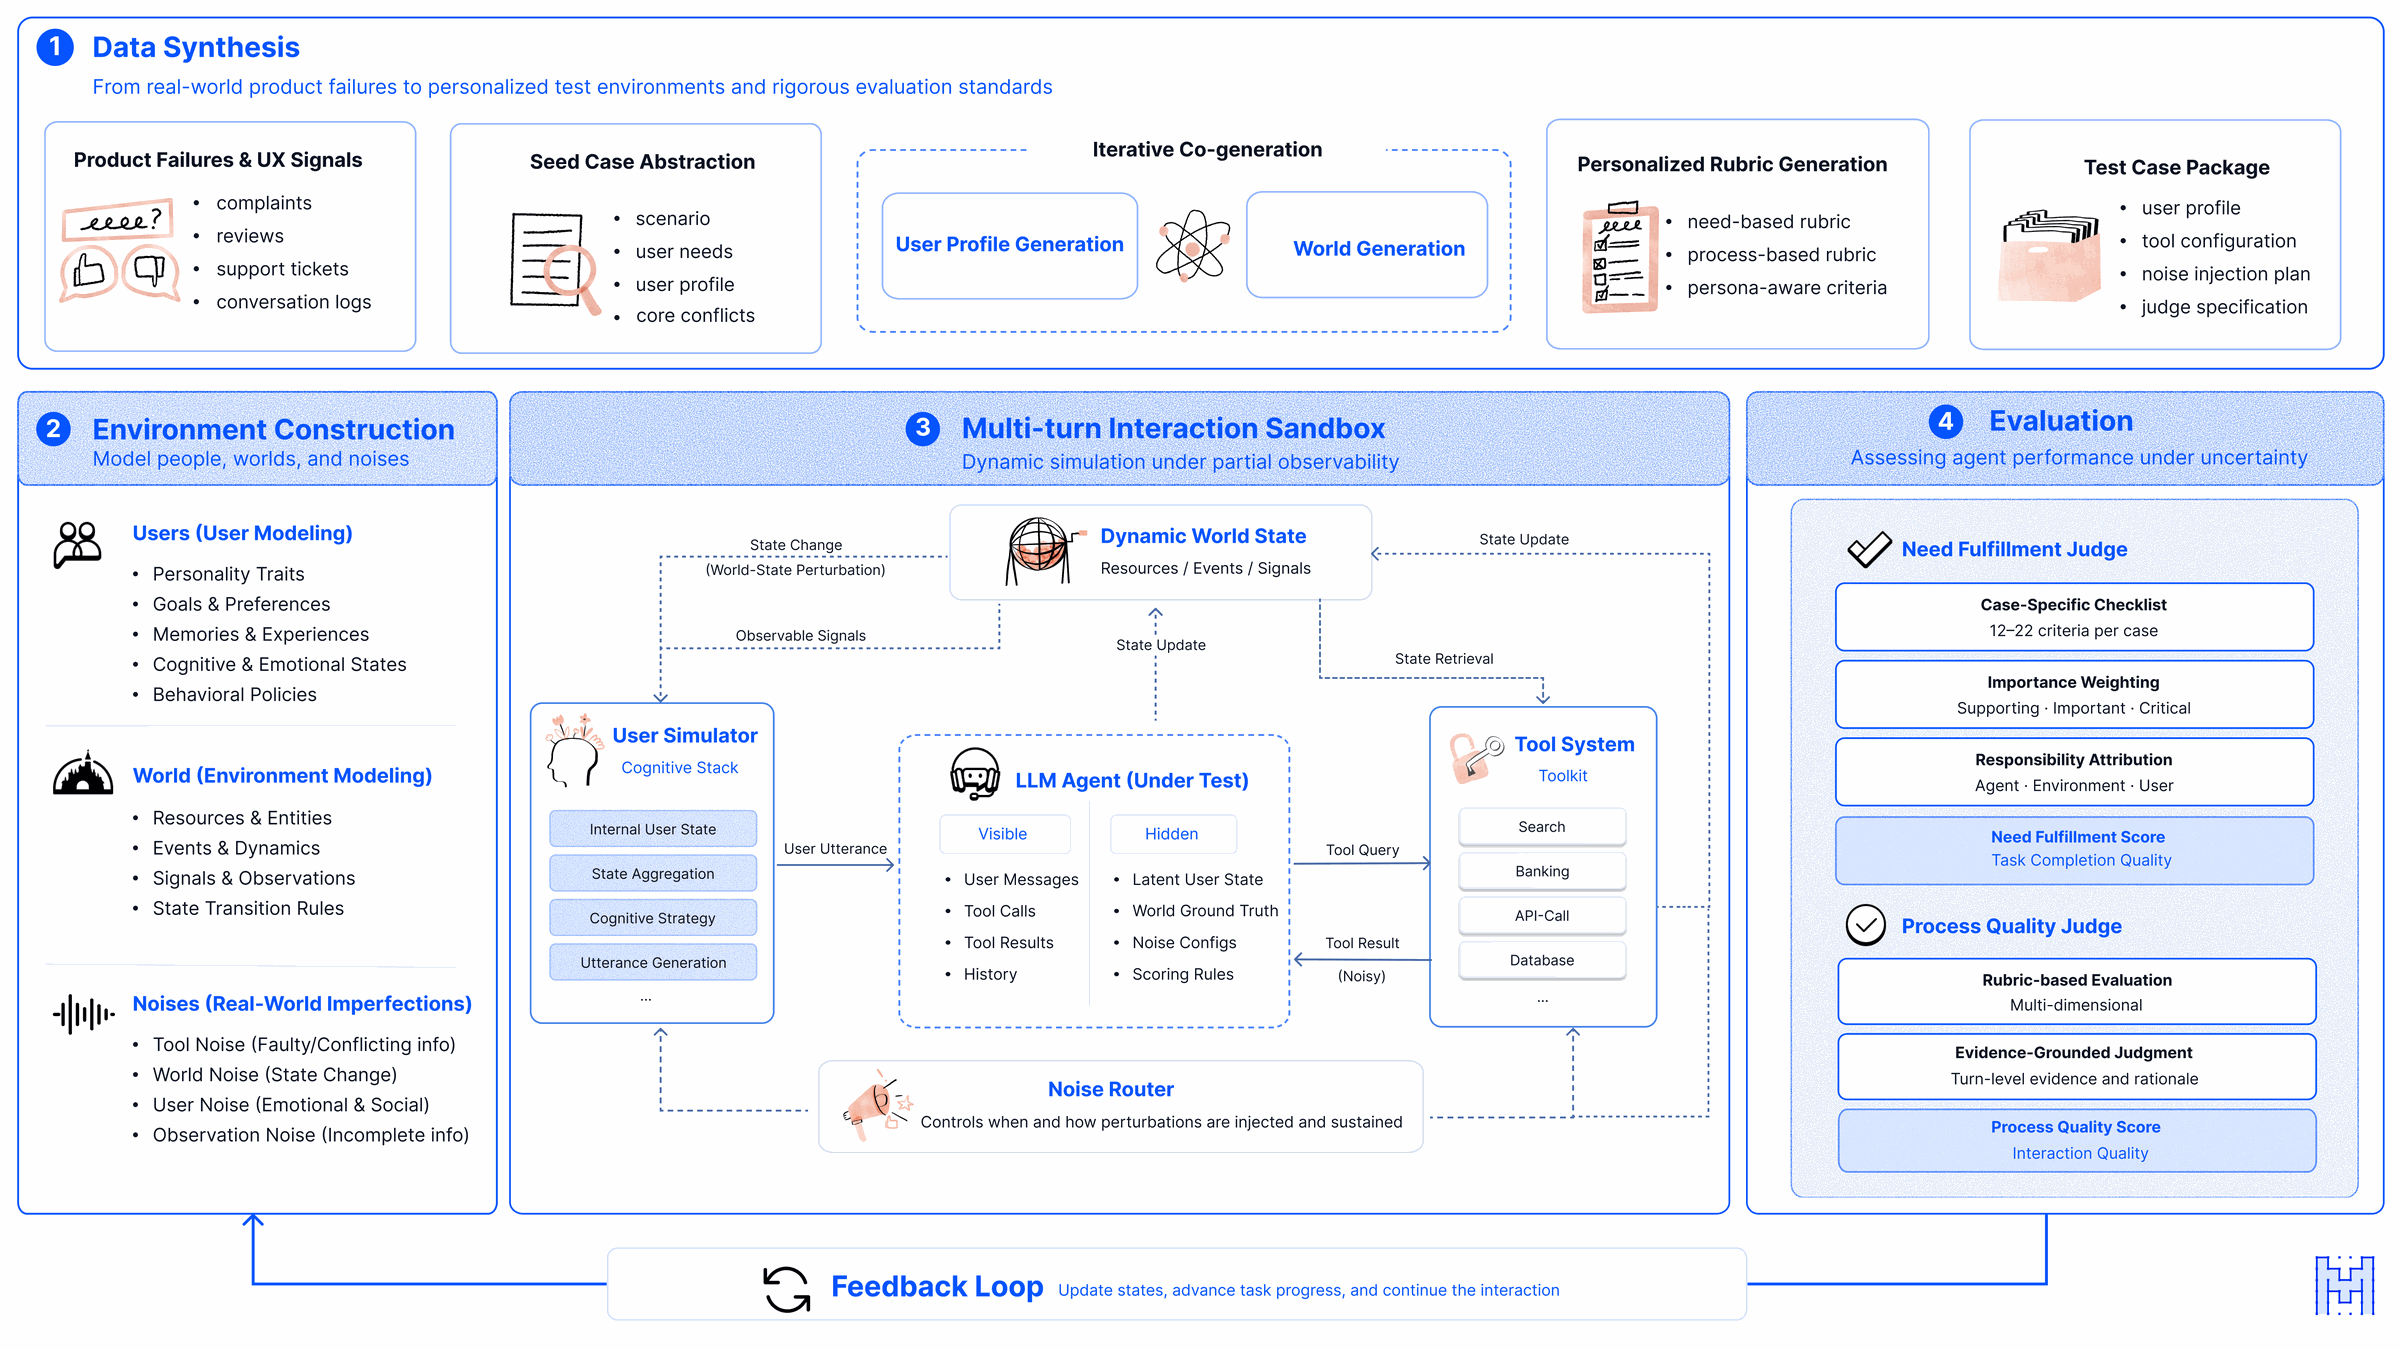
\includegraphics[width=\linewidth]{figures/livingbench_final.png}
\caption{\livingbench{} system architecture. Top: data synthesis from product failures to a case package. Bottom left: user, world, and noise construction. Bottom center: six-component interaction in the dynamic multi-agent sandbox. Bottom right: need-fulfillment and process-quality evaluation.}
\label{fig:livingbench}
\end{figure}

\subsubsection{Data Generation: One Seed, One World}
\label{sec:livingbench_datagen}

Each test case originates from analysis of failure taxonomies on product interactions. The construction process groups observed failures into system-level factors, such as tool failures, stale search results, conflicting sources, and infeasible constraint sets, and model-level factors, such as brittle requirement confirmation, failure to adapt when requirements change, and superficial agreement. These factors are represented through three parameter groups, namely persona, world constraints, and noise type.

Each case instantiates one combination of persona type, world background and constraints, and noise pattern. Multiple LLM calls expand this seed into a micro-world with hidden needs, resources, information gaps, a noise plan, and case-specific scoring criteria. Persona and environment are generated jointly so their constraints remain linked. The simulator then adapts its trajectory to each tested model, which supports closed-loop interaction but means different models need not receive identical event sequences.


\subsubsection{Four-Layer Noise System}
\label{sec:livingbench_noise}

Noise simulates information interference and environmental change in the real world. The system models four types, each testing different capabilities.

\paragraph{User noise} operates on the behavior layer, including time pressure, emotional fluctuations, social interference such as a superior assigning an urgent task, a child falling ill, or interpersonal tension causing volatility, and sudden preference changes. This tests judgment of life priorities and strategy adjustment.

\paragraph{World noise} operates on the fact layer, including resource changes such as sudden price increases or fully booked venues, unexpected events such as delayed flights or closed roads, and constraint changes. World facts have genuinely changed, testing adaptability and replanning.

\paragraph{Tool noise} operates on return values, including data tampering such as a rating of 4.8 tampered to 3.2, interface failures, and missing fields. World facts remain unchanged, with only tool-returned data corrupted. This tests information verification and cross-validation. When the model presents noise data as fact without verification, the system injects a visible recovery cue in the next turn, observing whether the model identifies the anomaly and re-queries.

\paragraph{Observation noise} operates on the model's visible information layer, including hidden or distorted observations, incomplete information, and multi-source contradictions, testing reasoning under information asymmetry.

The LLM-driven noise router decides each turn whether to release or withhold an event based on conversation progress. The same preset noise types, trigger windows, and routing rules are used for every model, while release timing follows each model's trajectory. The benchmark therefore compares complete model--simulator interactions under a common policy rather than replaying an identical fixed event sequence.

\subsubsection{Dynamic World Evolution}
\label{sec:livingbench_world}

Within the simulator, tool actions update world state, forming a tool $\to$ world $\to$ user chain. After a write operation such as rebooking a flight or sending a message, subsequent queries read the updated state. Some events are exposed immediately, while others are released when the relevant topic arises. This semantic simulation supports tests of replanning without constituting external-world execution.

The user simulator updates hidden psychological state turn by turn from world state and noise, and follows predefined information-disclosure strategies such as immediate, gradual, or withheld disclosure. At evaluation time, the tested model's interface exposes only public observations, not the simulator's hidden persona, world ground truth, or scoring checklist. This runtime separation ensures that every model acts only on benchmark-approved observations.

Evaluation uses two judge roles. The need judge makes binary decisions against a scenario-specific weighted checklist, while the process judge evaluates turn-level evidence for information integration, tool-use effectiveness, interaction quality, and proactive inquiry. The need checklist assigns each item one of three importance weights, namely supporting, important, or critical, and the need score is the weighted fraction of satisfied items, normalized to $[0,1]$. The process score is a weighted mean across the four process dimensions, each rated on a five-level scale; the per-turn mean is averaged across turns to an episode-level process score, also in $[0,1]$. A deterministic engine then combines these as $0.7\times$ need fulfillment $+\;0.3\times$ process quality, and the reported benchmark score is the macro-average of case scores scaled to $0$--$100$. Each model--case pair is run three times and averaged under the same simulator, judge stack, and aggregation rule.


\subsection{\uifora{}-Bench}
\label{sec:ui4abench}

Prior UI evaluations considered here primarily treat the interface either as an environment in which an agent acts, as in OSWorld~\citep{xie2024}, or as an artifact to compare with a reference design, as in Design2Code~\citep{si2025design2code}. A card generated inside a conversation need not have a unique visual reference. \uifora{}-Bench therefore measures whether a model can produce a clear, accurate, usable, and interactive card for the request under the standard \uifora{} runtime. The evaluation unit is the rendered card rather than an individual control or a screenshot-similarity target.

\subsubsection{Structure Visibility and Evaluation Set}
\label{sec:ui4a_visibility}

A card exists to turn the model's reasoning into a structured interface that users can directly read, correct, and continue using. We call the property supporting this \emph{structure visibility}. Rendering an interface rather than outputting a paragraph is worthwhile when it places the structure of information directly in front of the user, so they do not have to reconstruct it mentally. A successfully rendered card simultaneously fulfills five promises, namely answering the task, trustworthy content, clear structure, functional controls, and screen fit. These promises fail independently, so they are measured separately and combined.

The evaluation set contains 161 cases across eight experience domains, sourced from curated examples, de-identified production traffic, and coverage-gap sampling, with multilingual cases. Production-sourced prompts have a median length of approximately 790 characters and a maximum above 2{,}000 characters. These longer prompts test selection and hierarchy under information load. Because the set is deliberately curated rather than sampled to match deployment prevalence, the Final Score characterizes this case mix only.

\subsubsection{Evaluation Pipeline and Scoring}
\label{sec:ui4a_pipeline}

In the evaluation pipeline, the tested model emits React component source. The harness compiles it with a version-pinned toolchain and renders in headless Chromium at two viewports in parallel, mobile ($390\times844$) and desktop ($1440\times900$). Only the mobile viewport contributes to the primary visual evaluation, so the headline Final Score reflects mobile layout only. The evaluator records five Layer Scores.

\begin{figure}[t]
  \centering
  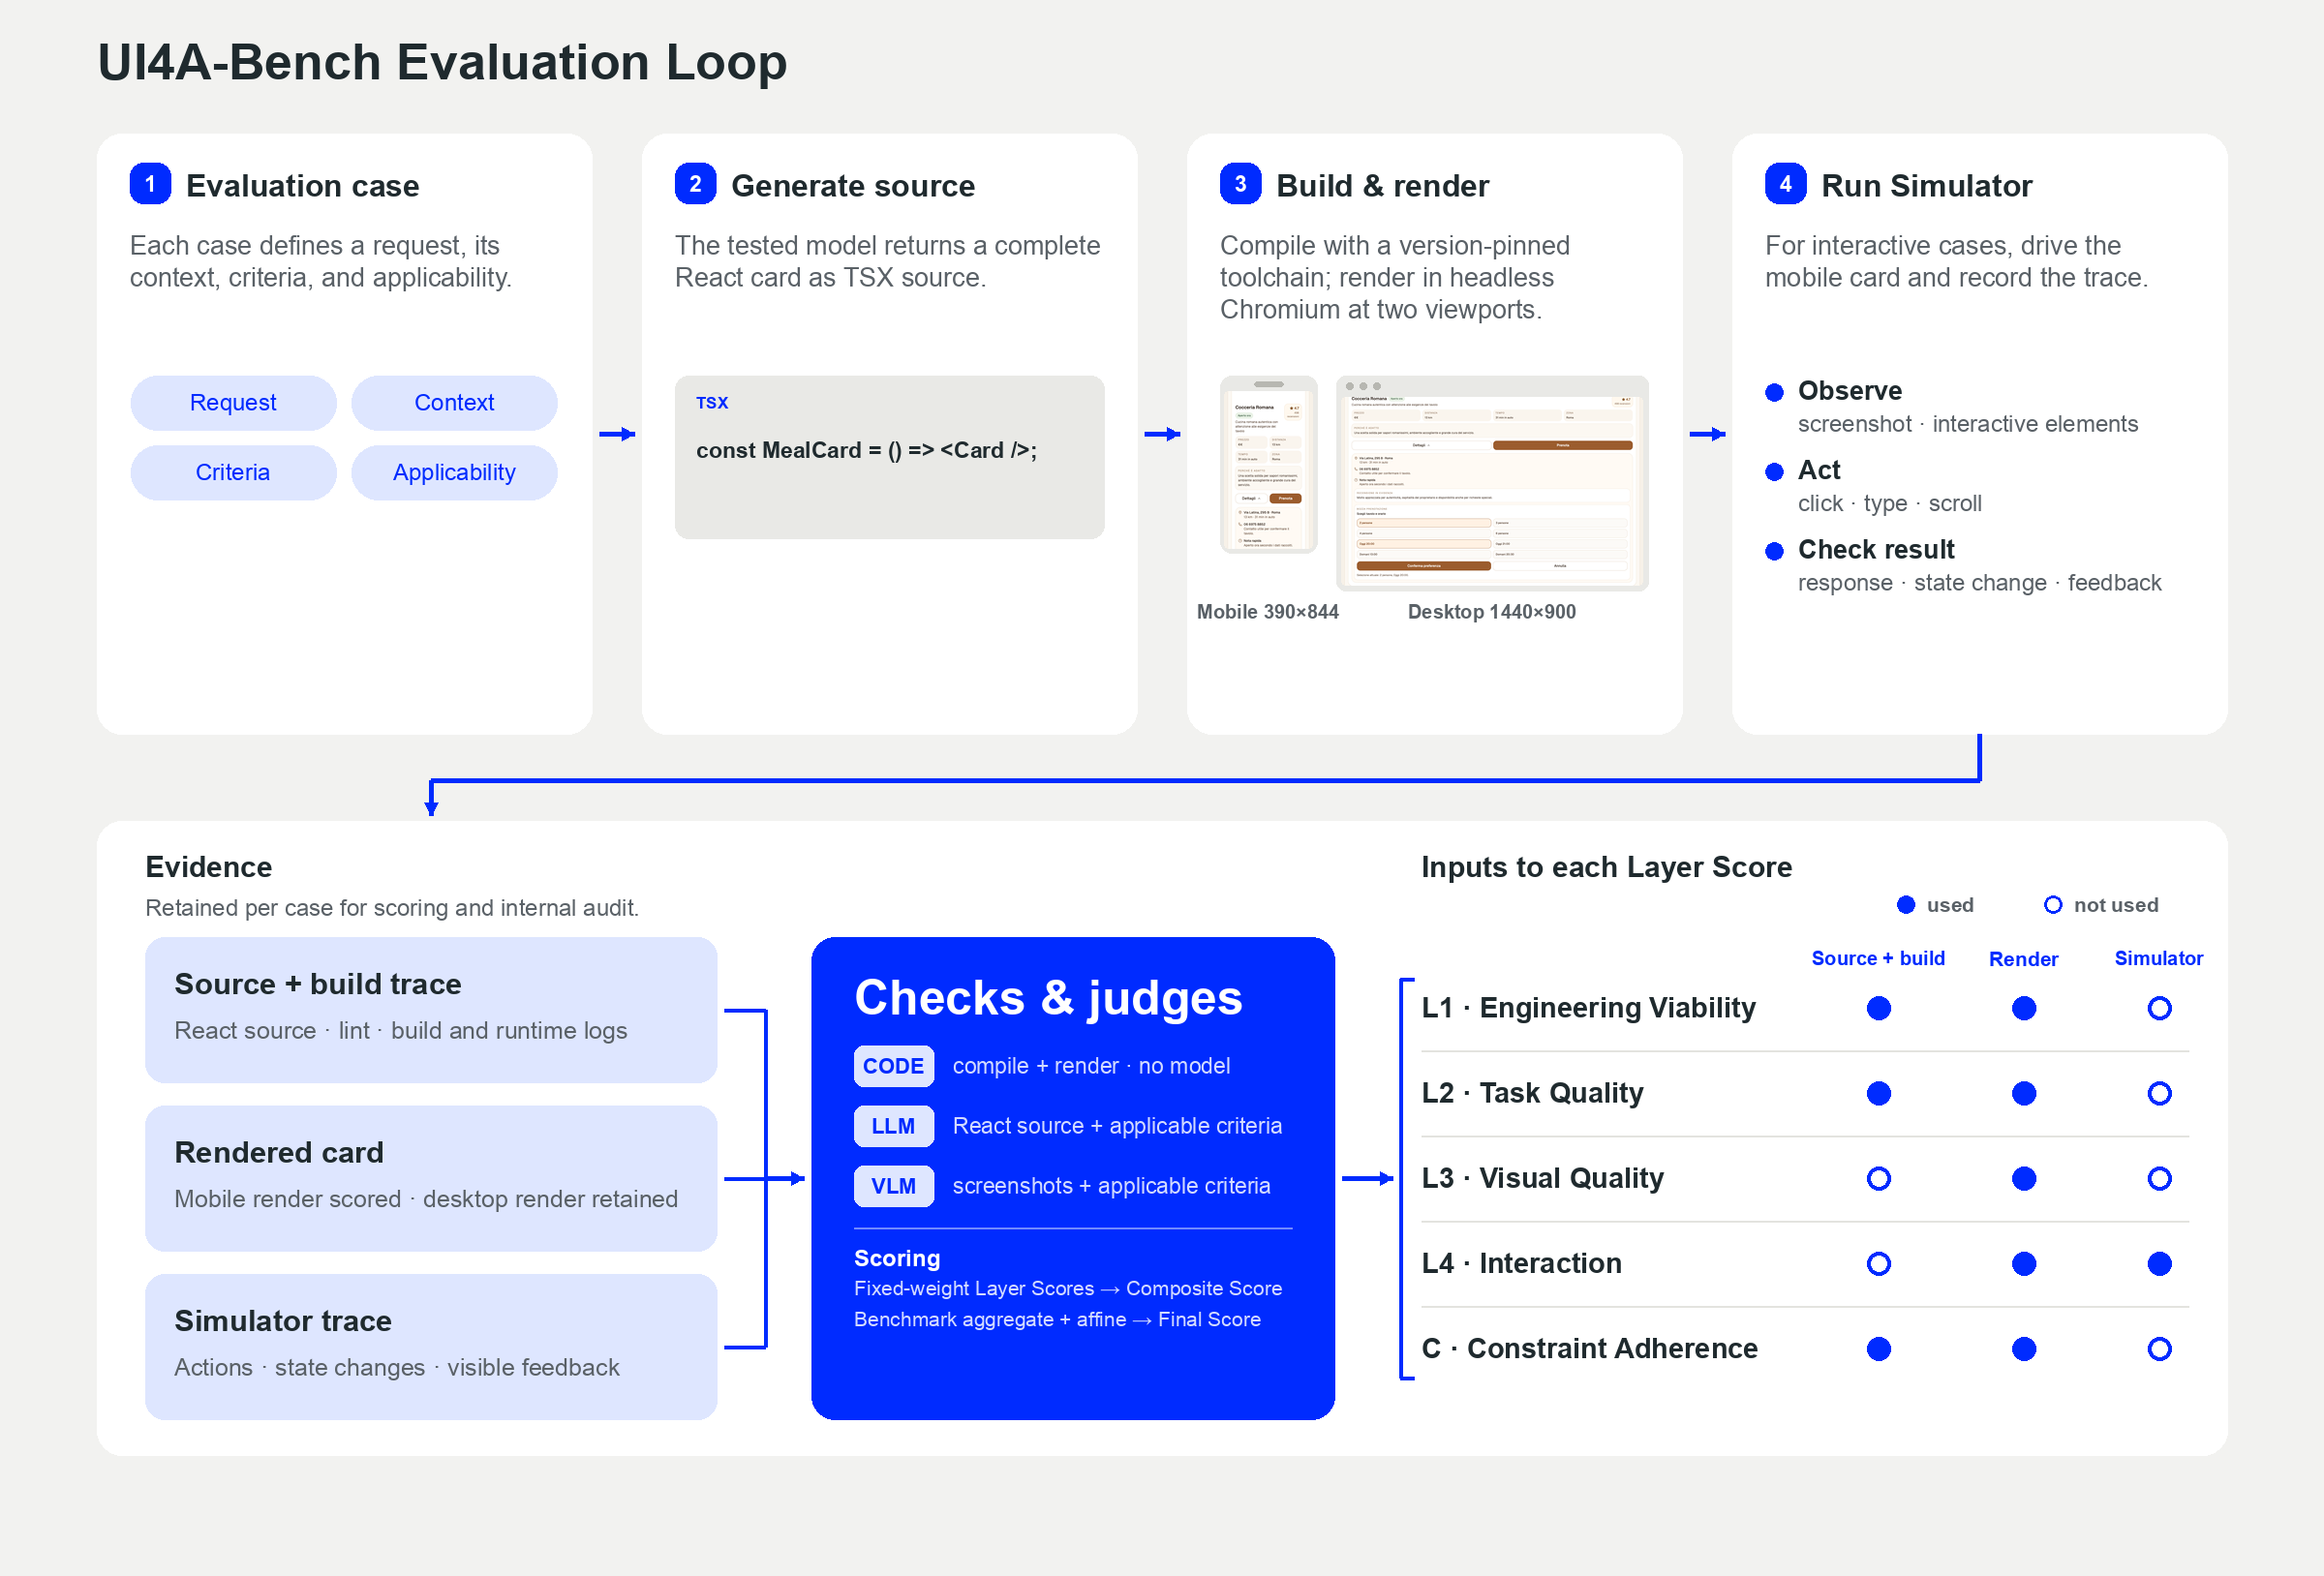
\includegraphics[width=\textwidth]{figures/ui4a_evaluation_loop.png}
  \caption{UI4A-Bench evaluation loop. Each case combines the request with relevant user context. The model generates a complete React card, which is compiled and rendered before the benchmark collects build, rendered, and browser-driven interaction evidence. Deterministic checks and evidence-based judges score the five reported Layer Scores.}
  \label{fig:ui4a_evaluation_loop}
\end{figure}

\begin{itemize}[leftmargin=*]
  \item \textbf{Engineering viability} measures whether the card compiles and renders without error, decidable with no model in the loop. All other dimensions depend on this.
  \item \textbf{Task quality} measures whether content correctly answers the user request, whether facts and figures are reliable, and whether the model fabricates when input is incomplete.
  \item \textbf{Visual quality} measures whether information hierarchy, emphasis, and mobile presentation allow the user to grasp the structure at a glance. Scored on task-anchored structure and legibility, not on style preference.
  \item \textbf{Interaction} measures whether controls respond, are wired to real state rather than decorative stubs, and whether the user sees feedback afterwards.
  \item \textbf{Constraint adherence} measures screen fit, coverage of explicitly mentioned requirements, and data grounding in the input rather than fabrication.
\end{itemize}

Interaction is evaluated by driving the rendered card in a headless browser. The evaluation agent clicks, types, and scrolls at the mobile viewport while observing screenshots and visible interactive elements. It records three observable criteria, whether a control responds, whether the action changes state, and whether feedback is visible afterwards. When a case declares an interaction requirement and the evaluator records no evidence, that requirement receives zero rather than being skipped.

The case set, generation configuration, scoring policy, and judge version are fixed across compared systems and recorded in a run manifest, with run artifacts and judge observations retained. Deterministic code combines the five Layer Scores with fixed weights into a Composite Score; the benchmark aggregate then passes through fixed, versioned affine normalization to produce the Final Score. A fixed observation set therefore maps to the same Final Score, and each reported run can be audited against its manifest.

\subsection{General Capability Benchmark Suite}
\label{sec:general_bench}

\chatbench{}, \livingbench{}, and \uifora{}-Bench target the release's specialized behavior, while the general-capability suite probes transfer to personal-life agent tasks, multi-step tool use, coding, and terminal operation. Matched comparisons such as \tall{} versus its base reveal differences on the measured tasks. In the broader \venti{} table, unstarred values are evaluated under a common protocol within each benchmark row; starred public values are included as contextual reference points.

The suite comprises VitaBench~\citep{vitabench2026} and PinchBench~\citep{pinchbench2026} for personal-life agent scenarios; ClawGym for multi-step tool composition; SWE-Verified~\citep{jimenez2024swebench}, DeepSWE~\citep{deepswe2026}, and SWE Atlas QnA~\citep{sweatlas2026} for coding; and TerminalBench 2.1~\citep{terminalbench2026} for terminal operation. Each row follows the benchmark-specific judge, scaffold, retry policy, and estimand (pass@1, pass@3, or best-of-run) documented in Appendix~\ref{app:eval_protocols}; this includes the reproduced GLM-5.1 evaluator used for VitaBench because its original judge is unavailable. Section~\ref{sec:results} marks values imported from external leaderboards. Scores are compared within benchmark rows rather than averaged across unlike metrics.
